% !TeX spellcheck = nl_NL
\documentclass[a4paper,kul]{kulakarticle} %options: kul or kulak (default)

\usepackage[utf8]{inputenc}
\usepackage[dutch]{babel}
\usepackage[T1]{fontenc}
\date{Academiejaar 2021 -- 2022}
\address{
	Industriële Ingenieurswetenschappen \\
	Trillingen \& Golven \\
	Maarten Vanierschot}
\title{Afleidingen}
\author{Robbe Decapmaker}
\usepackage{hyperref}
\usepackage{graphicx}
\usepackage{amsmath, amssymb, amsthm}
\usepackage{siunitx}
\usepackage{flafter} 
\usepackage{pdfpages}
\usepackage{pgfplots}
\usepackage{caption}
\usepackage{subcaption}

\begin{document}

\maketitle

\section*{Inleiding}

De afleidingen voor trillingen en golven. \href{https://github.com/debber1/Afleidingen_TG}{De source code is te vinden op github.}\\
https://github.com/debber1/Afleidingen\_TG\\
Dit document is \textbf{niet} alles wat je moet kennen van theorie voor het examen. Ik ben niet verantwoordelijk voor jouw resultaat op jouw examen. Het is jouw verantwoordelijkheid om ook nog de andere onderdelen van deze cursus op een degelijke manier te verwerken. \\
%DEZE ZIN IS ENKEL RELEVANT TIJDENS DE ONTWIKKELING VAN DIT DOCUMENT
\textbf{Dit document is een `work in progress', dit wil zeggen dat er (ongeveer) een wekelijkse update zal zijn. De meest recente versie zal altijd op Github staan!}

\section*{Contributors}
\href{https://github.com/sydon1}{Sodir Yuksel} \\
\href{https://github.com/ItsAlphie}{Jonathan Valgaeren}

\section{Afleiding 1}

\textbf{Uitdrukking voor de verplaatsing van een ongedempte trilling aan de hand van de bewegings-vergelijking}\\
\begin{figure}[htbp]
	\centering
	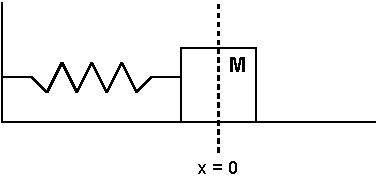
\includegraphics[width=0.4\linewidth]{MassaVeer}
	\caption[Massa veer systeem]{Massa veer systeem}
	\label{fig:massaveer}
\end{figure}
\begin{figure}[htbp]
	\centering
	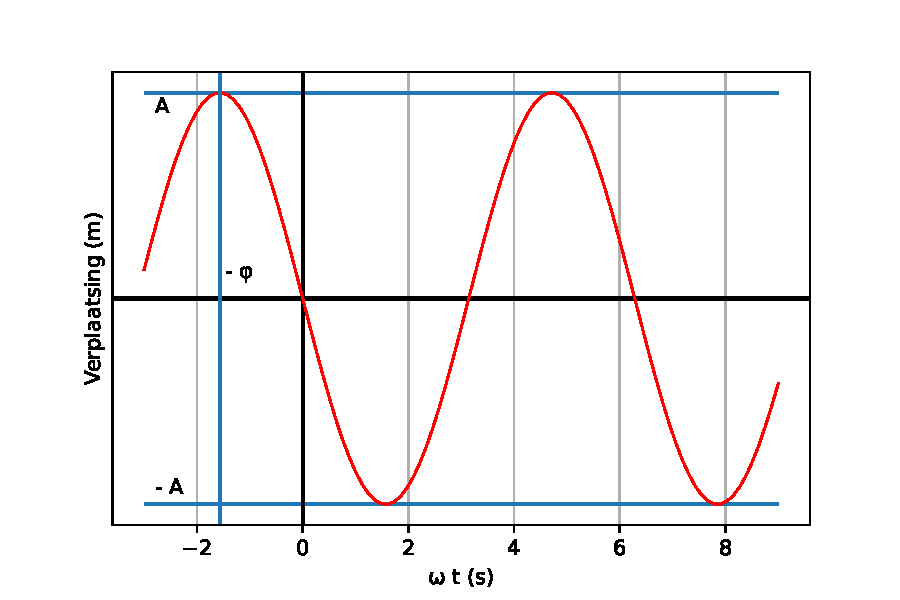
\includegraphics[width=0.7\linewidth]{Harmonische_Oscillator}
	\caption[Harmonische Oscillator]{Harmonische Oscillator}
	\label{fig:harmonischeoscilator}
\end{figure}

We stellen eerst de tweede wet van Newton op voor het blokje M uit figuur \ref{fig:massaveer}.
\begin{equation*}
	\sum \vec{F} = m\vec{a}
\end{equation*}
We kijken nu enkel naar de x-component en brengen de kracht van de veer in rekening:
\begin{equation*}
	-kx = m\frac{d^2x}{dt^2}
\end{equation*}
We hebben ook de versnelling geschreven als de tweede afgeleide van de verplaatsing. Door alle termen naar het linker lid te verplaatsen krijgen we volgende differentiaal vergelijking: 
\begin{equation}
	m\frac{d^2x}{dt^2} + kx = 0
	\label{eq:DVGLTrilling}
\end{equation}
Deze differentiaal vergelijking moeten we oplossen aan de hand van beginvoorwaarden. Deze voorwaarden verkrijgen we experimenteel. Bij het experiment noteren we de uitwijking tegenover de tijd. Hierdoor verkrijgen we figuur \ref{fig:harmonischeoscilator}.
Wiskundig vertaalt dit zich tot: 
\begin{equation}
	x(t) = A cos(\omega t + \varphi)
	\label{eq:trilling}
\end{equation}
We kunnen vergelijking \ref{eq:trilling} een eerste keer afleiden om de snelheid van het blokje te verkrijgen: 
\begin{equation}
	v(t) = \frac{dx(t)}{dt} = -\omega Asin(\omega t + \varphi)
	\label{eq:trillingsnelheid}
\end{equation}
Door vergelijking \ref{eq:trilling} nogmaals af te leiden, kunnen we ook de versnelling van het blokje verkrijgen:
\begin{equation}
	a(t) = \frac{d^2x(t)}{dt^2} = -\omega^2 Acos(\omega t + \varphi)
	\label{eq:trillingversnelling}
\end{equation}
Nu kunnen we vergelijkingen \ref{eq:trillingversnelling} en \ref{eq:trilling} invullen in vergelijking \ref{eq:DVGLTrilling}:
\begin{equation}
	-\omega^2 mAcos(\omega t + \varphi) + k A cos(\omega t + \varphi) = 0
	\label{eq:Bewegingsvergelijking}
\end{equation}
Vergelijking \ref{eq:Bewegingsvergelijking} is nu een oplossing voor differentiaal vergelijking \ref{eq:DVGLTrilling} als aan volgende voorwaarde voldaan is:
\begin{align*}
	-\omega^2 mAcos(\omega t + \varphi) + k A cos(\omega t + \varphi) & = 0\\
	(\frac{k}{m}-\omega^2)A cos(\omega t + \varphi) & = 0\\
	\frac{k}{m}-\omega^2 & = 0\\
	\frac{k}{m} & = \omega^2
\end{align*}


\newpage
\section{Afleiding 2}
\textbf{Potentiële en kinetische energie van een ongedempte trilling in functie van de plaats}
\\

Er zijn 2 vormen van energie aanwezig in een massa-veer-systeem. We hebben de potentiële energie in de veer en de kinetische energie van het blokje.
\begin{align*}
	E = & \frac{1}{2}kx^2 + \frac{1}{2}mv^2\\
	E(x) = & \frac{1}{2}k A^2cos^2(\omega t +\varphi) + \frac{1}{2}m \omega^2 A^2 sin^2(\omega t + \varphi)\\
	E(x) = & \frac{1}{2}k A^2cos^2(\omega t +\varphi) + \frac{1}{2}m \frac{k}{m} A^2 sin^2(\omega t + \varphi)\\
	E(x) = & \frac{1}{2} k A^2 (cos^2(\omega t +\varphi) + sin^2(\omega t + \varphi))\\
	E(x) = & \frac{1}{2} k A^2
\end{align*} 
We zien nu duidelijk dat de hoeveelheid energie niet afhankelijk is van de uitwijking van de massa. Met andere woorden: de energie blijft constant in het systeem (figuur \ref{fig:energiebalans}).
\begin{figure}[htbp]
	\centering
	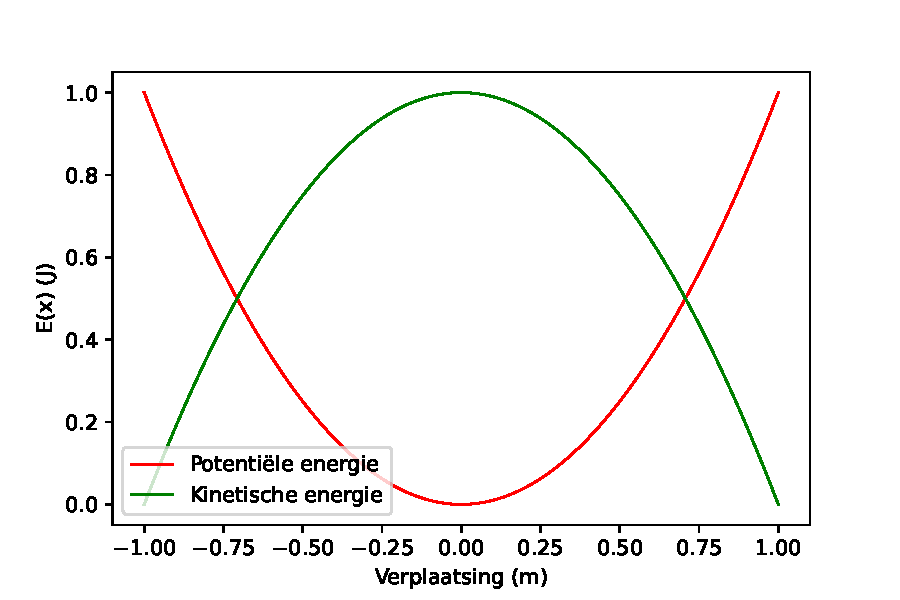
\includegraphics[width=0.7\linewidth]{Energie_Balans}
	\caption[Energie balans]{Energie balans}
	\label{fig:energiebalans}
\end{figure}

\newpage

\section{Afleiding 3}
\textbf{Snelheid in functie van de afstand}
\begin{equation*}
	\frac{dv}{dt} = \frac{dv}{dx}\cdot\frac{dx}{dt}
\end{equation*}
We kunnen vergelijkingen \ref{eq:trilling} en \ref{eq:trillingsnelheid} invullen:
\begin{equation*}
	-A\omega^2cos(\omega t + \varphi) = \frac{dv}{dx}\cdot A\omega sin(\omega t +\varphi)
\end{equation*}
Na schrappen en herschikken:
\begin{equation*}
	\frac{dv}{dx} = \frac{\omega cos(\omega t + \varphi)}{sin(\omega t + \varphi)}
\end{equation*}
Sinus substitutie:
\begin{align*}
	\frac{dv}{dx} =& \frac{\omega cos(\omega t + \varphi)}{\sqrt{1-cos^2(\omega t + \varphi)}}\\
	\frac{dv}{dx} =& \frac{\pm \omega \frac{x}{A}}{\sqrt{1-\frac{x^2}{A^2}}}
\end{align*}
Nu integratie van beide leden:
\begin{equation*}
	\int dv = \int \frac{\pm \omega \frac{x}{A}}{\sqrt{1-\frac{x^2}{A^2}}} dx
\end{equation*}
De snelheid in functie van de afstand is dus:
\begin{equation}
	\label{eq:snelheid_positie}
	v(x) = \omega A\sqrt{1-\frac{x^2}{A^2}}
\end{equation}
Uit vergelijking \ref{eq:snelheid_positie} kunnen we nu ook afleiden wat de uitdrukking is voor $v_{\text{max}}$. We weten dat $v_{\text{max}}$ zich zal voordoen bij het evenwichtspunt oftewel als x = 0.
\begin{align*}
	v(x) =& \omega A\sqrt{1-\frac{x^2}{A^2}}\\
	v_{\text{max}} =& \omega A\sqrt{1-\frac{0^2}{A^2}}\\
	v_{\text{max}} =& \omega A\sqrt{1}\\
	v_{\text{max}} =& \omega A
\end{align*}
\newpage
\section{Afleiding 4}
\textbf{Beweging van een pendulum aan de hand van de bewegingsvergelijking}
\begin{figure}[htbp]
	\centering
	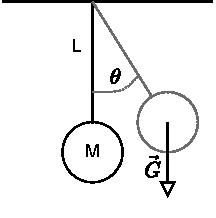
\includegraphics[width=0.5\linewidth]{Pendulum}
	\caption[Pendulum]{Pendulum}
	\label{fig:pendulum}
\end{figure} \\
De drijvende kracht van de pendulum is gelijk aan:
\begin{equation*}
	F = -mg sin(\theta)
\end{equation*}
Hiermee kunnen we de bewegingsvergelijking opstellen:
\begin{equation*}
	m\frac{d^2x}{dt^2} = -mgsin(\theta)
\end{equation*}
We kunnen stellen dat $sin(\theta) \approx \theta$ voor een kleine $\theta$:
\begin{equation*}
	m\frac{d^2x}{dt^2} = -mg\theta
\end{equation*}
We kunnen ook stellen dat $x = l\theta$:
\begin{equation*}
	ml\frac{d^2\theta}{dt^2} = -mg\theta
\end{equation*}
We kunnen dit nu herschrijven naar:
\begin{equation*}
	\frac{d^2\theta}{dt^2} +\frac{g}{l}\theta = 0
\end{equation*}
Dit geeft ons een differentiaalvergelijking. Een oplossing ziet er als volgt uit:
\begin{equation*}
	\theta (t) = \theta_0 cos(\omega t +\varphi)
\end{equation*}
Hierbij zien we dat $\omega = \sqrt{\frac{g}{l}}$.
\newpage
\section{Afleiding 5}
\textbf{Gedempte harmonische trilling}\\
\begin{figure}[htbp]
	\centering
	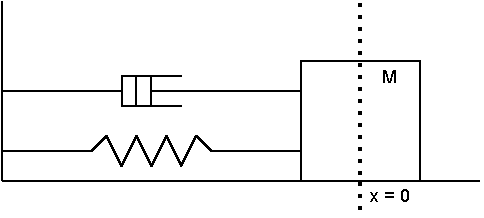
\includegraphics[width=0.7\linewidth]{DempingVeer}
	\caption[Gedempt massa veer systeem]{Gedempt massa-veer-systeem}
	\label{fig:dempingveer}
\end{figure}
We beginnen met de bewegingsvergelijking op te stellen:
\begin{align*}
	m \vec{a} =& \vec{F}_{veer} + \vec{F}_{demper}\\
	m \frac{d^2x}{dt^2} = & -kx - bv\\
	m \frac{d^2x}{dt^2} = & -kx - b\frac{dx}{dt}\\
	0 = & m \frac{d^2x}{dt^2} + b\frac{dx}{dt} + kx
\end{align*}
We maken gebruik van de formule van Euler $e^{i\varphi}=cos(\varphi) +isin(\varphi)$ om tot een oplossing van de differentiaalvergelijking te komen:
\begin{equation*}
	\widetilde{x}(t) = Ae^{(\gamma +i\omega)t+i\varphi}
\end{equation*}
Het reëel deel is dus:
\begin{equation*}
	x(t) = Re(\widetilde{x}(t)) = Ae^{\gamma t}cos(\omega t + \varphi)
\end{equation*}
We kunnen deze nu invullen in de bewegingsvergelijking:
\begin{equation}
	\label{eq:complexbeweging}
	m(\gamma +i\omega)^2\widetilde{x}(t) + b(\gamma +i\omega)e^{(\gamma +i\omega)t+i\varphi}+ke^{(\gamma +i\omega)t+i\varphi} = 0
\end{equation}
Na herordenen en het delen door m, krijgen we:
\begin{equation*}
	\gamma^2+2i\gamma\omega-\omega^2+\frac{b}{m}\gamma+i\frac{\omega b}{m}+\frac{k}{m}=0
\end{equation*}
We kijken nu naar het imaginair deel:
\begin{align*}
	2i\gamma \omega +i\frac{\omega b}{m}&=0\\
	2\gamma + \frac{b}{m} = 0\\
	-\frac{b}{2m} = \gamma
\end{align*}
We vullen nu deze waarde van $\gamma$ in in het reëel deel van vergelijking \ref{eq:complexbeweging}:
\begin{align*}
	\gamma^2-\omega^2+\frac{b}{m}\gamma+\frac{k}{m} &=0\\
	(-\frac{b}{2m})^2-\omega^2+\frac{b}{m}(-\frac{b}{2m})+\frac{k}{m} &=0\\ 
	\frac{k}{m}-\frac{b^2}{4m^2}&=\omega^2\\
	\sqrt{\frac{k}{m}-\frac{b^2}{4m^2}}&=\omega
\end{align*}
Hiermee hebben we nu de natuurlijke frequentie van het systeem gevonden. We kunnen tot slot ook nog stellen dat:
\begin{equation*}
	x(t) = Re(\widetilde{x}(t)) = Ae^{-\frac{b}{2m} t}cos(\omega t + \varphi)
\end{equation*}
We kunnen nu drie gevallen onderscheiden: 
\begin{figure}[htbp]
	\centering
	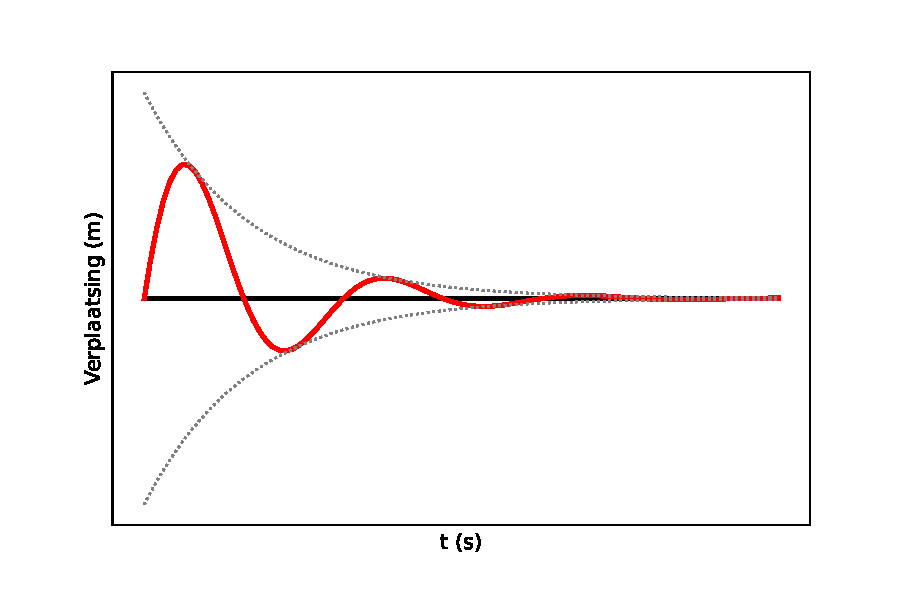
\includegraphics[width=0.6\linewidth]{Ondergedempt}
	\caption[Ondergedempte trilling]{Ondergedempte trilling ($b^2 << 4mk$)}
	\label{fig:ondergedempt}
\end{figure}
\begin{figure}[htbp]
	\centering
	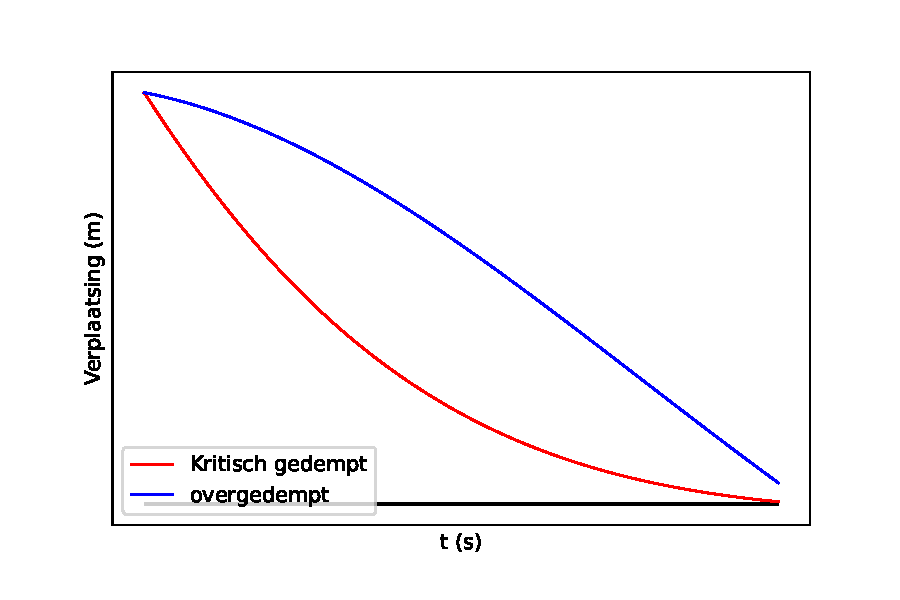
\includegraphics[width=0.6\linewidth]{Over_Kritisch_gedempt}
	\caption[Kritisch en over gedempte trilling]{Kritisch ($b^2 = 4mk$) en over gedempte ($b^2 >> 4mk$) trilling}
	\label{fig:overkritischgedempt}
\end{figure}


\newpage
\section{Afleiding 6}
\textbf{Gedwongen trillingen}\\
We stellen eerst de bewegingsvergelijking op:
\begin{equation}
	m\frac{d^2\widetilde{x}(t)}{dt^2}+b\frac{d\widetilde{x}(t)}{dt}+k\widetilde{x}(t) = F_0cos(\omega t)
	\label{eq:gedwongenbewegings}
\end{equation}
Een voorstel voor de algemene oplossing van differentiaalvergelijking \ref{eq:gedwongenbewegings} ziet er als volgt uit:
\begin{equation*}
	\widetilde{x}(t) = Ae^{i(\omega t +\varphi)}
\end{equation*}
waarbij $\widetilde{F} = F_0e^{i\omega t}$.
Dit kunnen we nu invullen in vergelijking \ref{eq:gedwongenbewegings}:
\begin{align*}
	m\omega^2\widetilde{x}(t)+i\omega b\widetilde{x}(t)+k\widetilde{x}(t) & =F_0e^{i\omega t}\\
	m\omega^2A^{i\omega t}e^{i\varphi}+i\omega bA^{i\omega t}e^{i\varphi}+kA^{i\omega t}e^{i\varphi} & =F_0e^{i\omega t}\\
	m\omega^2A+i\omega b+k & =F_0e^{-i\varphi} 
\end{align*}
We kunnen dit opsplitsen in een imaginair en reëel deel:
\begin{description}
	\item[Imaginair:]$\omega bA = -F_0sin(\varphi)$
	\item[Reëel:] $-m\omega A +kA = F_0cos(\varphi)$
\end{description}
Als we nu het imaginair deel delen door het reëel deel verkrijgen we voor $\varphi$:
\begin{align*}
	-\frac{\omega b}{k-m\omega^2} &= tan(\varphi)\\
	bgtan(\frac{-\omega b}{k-m\omega^2}) & =\varphi
\end{align*}
Om de amplitude te bepalen kijken we opnieuw naar het imaginair deel:
\begin{align*}
	\omega bA &= -F_0sin(\varphi)\\
	\omega bA &= -F_0\frac{tan(\varphi)}{\sqrt{1+tan^2(\varphi)}}\\
	\omega bA &= -F_0\frac{tan(bgtan(\frac{-\omega b}{k-m\omega^2}))}{\sqrt{1+tan^2(bgtan(\frac{-\omega b}{k-m\omega^2}))}}\\
	\omega bA &= -F_0\frac{\frac{-\omega b}{k-m\omega^2}}{\sqrt{1+\frac{\omega^2 b^2}{(k-m\omega^2)^2}}}\\
	\omega bA &= -F_0\frac{\frac{-\omega b}{k-m\omega^2}}{\sqrt{\frac{(k-m\omega^2)^2+\omega^2 b^2}{(k-m\omega^2)^2}}}\\
	A &= \frac{\frac{F_0}{k-m\omega^2}}{\sqrt{\frac{(k-m\omega^2)^2+\omega^2 b^2}{(k-m\omega^2)^2}}}\\
	A &= \frac{\frac{F_0}{m}}{\sqrt{(\frac{k}{m}-\omega^2)^2+\frac{\omega^2b^2}{m^2}}}\\
	A &= \frac{\frac{F_0}{m}}{\sqrt{(\omega_0^2-\omega^2)^2+\frac{\omega^2b^2}{m^2}}}	
\end{align*}
met $\omega_0$ de natuurlijke frequentie van het systeem en $\omega$ de gedwongen frequentie.
\newpage
\section{Afleiding 7}
\textbf{Golf vergelijking}\\
We nemen aan da $F_r$ en $F_l$ uit figuur \ref{fig:touwgolf} gelijk zijn aan elkaar en aan de spanning in het touw $\sigma A$. we stellen ook dat de massa voldoet aan $dm=\rho dsA$.\\
\begin{figure}[htbp]
	\centering
	\includegraphics[width=0.7\linewidth]{"touw_golf"}
	\caption[Touw]{Touw}
	\label{fig:touwgolf}
\end{figure}\\
We starten met het opstellen van de wet van Newton:
\begin{align*}
	\sum\vec{F}&=m\vec{a}\\
	F_rsin(\alpha_r) & = F_lsin(\alpha_l) = dma_y\\
	\sigma A(sin(\alpha_r)-sin(\alpha_l)) & = dm\frac{\partial^2y}{\partial t^2}\\
	\sigma(\frac{dy}{dx}|_r-\frac{dy}{dx}|_l) & = \rho ds \frac{\partial^2y}{\partial t^2}
\end{align*}
We stellen dat $\alpha$ klein is, en dus kunnen we zeggen dat $sin(\alpha)\approx tan(\alpha) = \frac{dx}{dy}$. We nemen ook aan dat $ds \approx dx$.
\begin{align*}
	\sigma\frac{\frac{dy}{dx}|_r-\frac{dy}{dx}|_l}{dx} & = \rho \frac{\partial^2y}{\partial t^2}\\
	\sigma\frac{\partial^2y}{\partial x^2} & = \rho \frac{\partial^2y}{\partial t^2}\\
	\frac{\partial^2y}{\partial t^2} & = \frac{\sigma}{\rho}\frac{\partial^2y}{\partial x^2}\\
	\frac{\partial^2y}{\partial t^2} & = v^2\frac{\partial^2y}{\partial x^2}
\end{align*}
Hiermee zijn we de 1D golfvergelijking bekomen.
\newpage
\section{Afleiding 8}
\textbf{Harmonische golven}\\
Een voorstel voor de 1D golf vergelijking ziet er als volgt uit:
\begin{equation*}
	y(x,t) = y_msin(kx \pm \omega t +\varphi)
\end{equation*}
We kunnen deze oplossing invullen in de golfvergelijking:
\begin{equation*}
	-\omega^2y_msin(kx \pm \omega t +\varphi)=v^2k^2y_msin(kx \pm \omega t +\varphi)
\end{equation*}
Als we dit vereenvoudigen, krijgen we de voorwaarden waaraan een golf moet voldoen.
\begin{align*}
	v^2 & = \frac{\omega^2}{k^2}\\
	v & = \pm\frac{\omega}{k}
\end{align*}
We kunnen nu een analyse doen op de golfvergelijking in het tijdsdomein:\\
\begin{figure}[h]
	\centering
	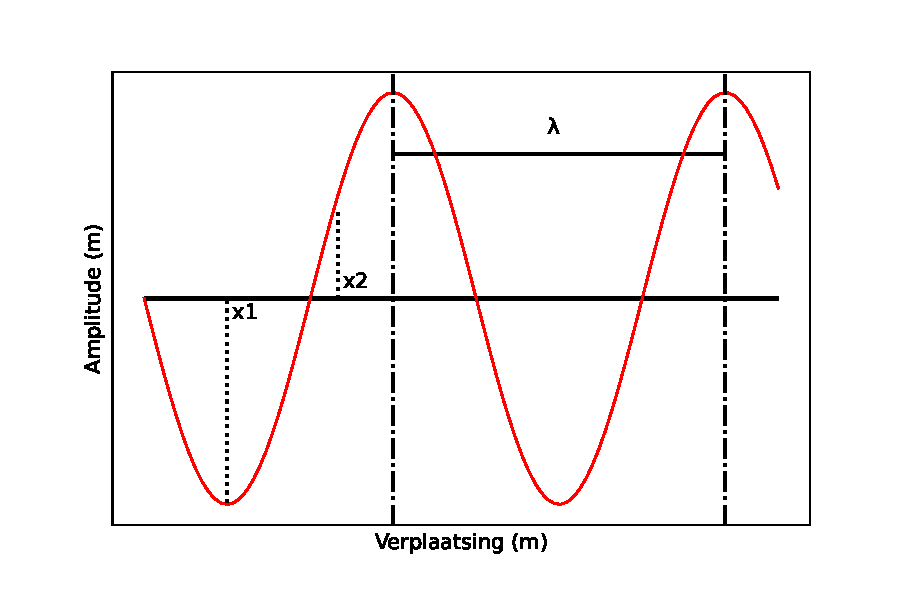
\includegraphics[width=0.7\linewidth]{tijdsdomein_analyse}
	\caption[Tijdsdomein analyse]{Tijdsdomein analyse}
	\label{fig:tijdsdomein}
\end{figure}\\
We starten opnieuw met de algemene oplossing, maar dan op vaste plaats $x_1$:
\begin{align}
	y(x_1,t) &= y_msin(kx_1 \pm \omega t +\varphi)\\
	\label{eq:tijdsanalyse1}
	y(x_1,t) &= y_msin(\pm \omega t +\varphi_1)
\end{align}
met $\varphi_1 = kx_1 +\varphi$. We kunnen dit opnieuw doen voor $x_2$:
\begin{align}
	y(x_2,t) &= y_msin(kx_2 \pm \omega t +\varphi)\\
	\label{eq:tijdsanalyse2}
	y(x_2,t) &= y_msin(\pm \omega t +\varphi_2)
\end{align}
met $\varphi_2 = kx_2 +\varphi$. Uit vergelijkingen \ref{eq:tijdsanalyse1} en \ref{eq:tijdsanalyse2} stellen we vast dat er enkel een fase verschuiving is. We vermelden ook nog dat oscillaties in fase zijn als $2\pi = k\lambda$.
\newpage
We doen ook de analyse doen op de golfvergelijking in de ruimte:\\
\begin{figure}[h]
	\centering
	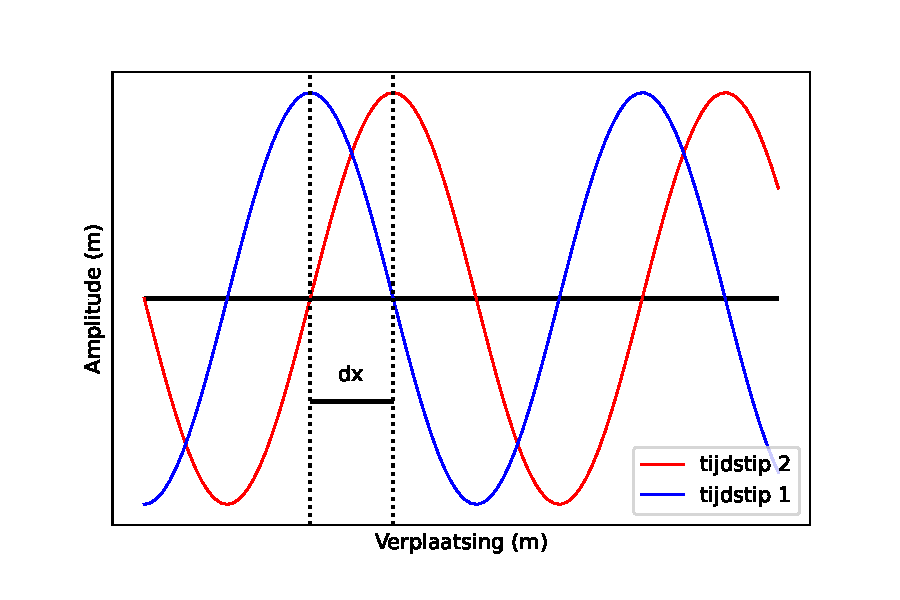
\includegraphics[width=0.7\linewidth]{ruimtelijke_analyse}
	\caption[Ruimtelijke analyse]{Ruimtelijke analyse}
	\label{fig:ruimtelijkeanalyse}
\end{figure}\\
We starten opnieuw met de algemene oplossing, maar dan op vast tijdstip $t_1$:
\begin{align}
	y(x,t_1) &= y_msin(kx \pm \omega t_1 +\varphi)\\
	\label{eq:ruimteanalyse1}
	y(x,t_1) &= y_msin(kx +\varphi_1)
\end{align}
met $\varphi_1 = \varphi \pm \omega t_1$. We stellen dit opnieuw op voor $t_2$
\begin{align}
	y(x,t_2) &= y_msin(kx \pm \omega t_2 +\varphi)\\
	y(x,t_2) &= y_msin(kx \underbrace{\pm \omega t_1 +\varphi}_{\varphi_1}\pm\Delta t)\\
	\label{eq:ruimteanalyse2}
	y(x,t_2) &= y_msin(kx +\varphi_2)
\end{align}
met $\varphi_2 = \varphi_1\pm\Delta t$.
Uit de waarden van $\varphi_1$ en $\varphi_2$ kunnen we de voortplantingsrichting van de golf bepalen: 
\begin{center}
	\begin{tabular}{|c|c|}
		\hline
		$\varphi_1$ < $\varphi_2$& Golf naar rechts \\
		\hline
		$\varphi_1$ > $\varphi_2$& Golf naar links \\
		\hline
	\end{tabular} 
\end{center}
We kunnen ook iets zeggen over de voortplantingssnelheid $v$.
\begin{align*}
 v = \frac{dx_{max}}{dt} = \frac{d}{dt}(kx_{max} \pm \omega t +\varphi) &= 0\\
 k\frac{dx_{max}}{dt}\pm \omega & = 0\\
 \pm \frac{\omega}{k} & = v\\
 \pm\frac{2\pi f}{\frac{2\pi}{\lambda}} & = v\\
 \pm \lambda f & = v
\end{align*}
\newpage
\section{Afleiding 9}
\textbf{Superpositie}\\
We zeggen dat de algemene oplossing $y(x,t)$ van de golfvergelijking kan uitgedrukt worden door 2 nieuwe functies:
\begin{equation*}
	y(x,t) = y_1(x,t)+y_2(x,t)
\end{equation*}
We vullen dit opnieuw in in de golfvergelijking:
\begin{align*}
	\frac{\partial^2 y(x,t)}{\partial t^2} & = v^2 \frac{\partial^2 y(x,t)}{\partial x^2}\\
	\frac{\partial^2 y_1(x,t)+y_2(x,t)}{\partial t^2} & = v^2 \frac{\partial^2 y_1(x,t)+y_2(x,t)}{\partial x^2}\\
\end{align*}
We gebruiken de lineariteit van de afgeleide:
\begin{equation*}
	\frac{\partial^2 y_1(x,t)}{\partial t^2} +\frac{\partial^2 y_2(x,t)}{\partial t^2}  = v^2(\frac{\partial^2 y_1(x,t)}{\partial x^2}+\frac{\partial^2 y_2(x,t)}{\partial x^2})
\end{equation*}
\newpage
\section{Afleiding 10}
\textbf{Interferentie}\\
Interferentie doet zich voor als er meerdere verschillende golven aanwezig zijn in 1 medium. We kunnen dit voorstellen door volgende 2 functies (zie ook figuur \ref{fig:interferentie}):
\begin{align*}
	y_1 & = y_msin(kx\pm\omega t)\\
	y_2 & = y_msin(kx\pm\omega t +\phi)
\end{align*}
\begin{figure}[h]
	\centering
	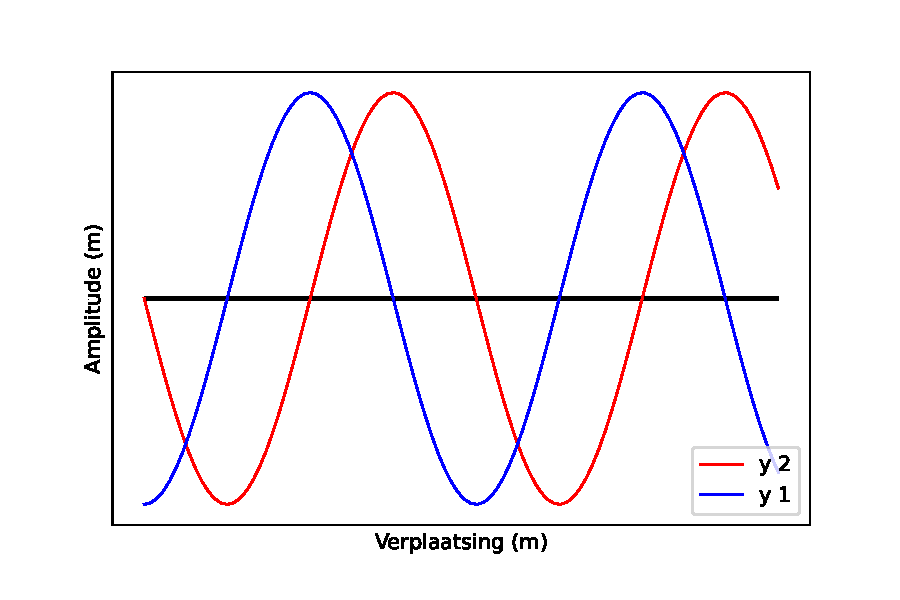
\includegraphics[width=0.5\linewidth]{Interferentie}
	\caption[Interferentie]{Golven $y_1$ en $y_2$ die zullen interfereren}
	\label{fig:interferentie}
\end{figure}\\
We bepalen nu hoe $y_1+y_2$ er wiskundig uit zal zien a.d.h.v. de \href{https://nl.wikipedia.org/wiki/Lijst_van_goniometrische_gelijkheden#Som-naar-product-identiteiten_(regels_van_Simpson)}{regels van Simpson}:
\begin{align*}
	y & = y_1+y_2\\
	y & = y_msin(kx\pm\omega t) y_m+sin(kx\pm\omega t +\phi)\\
	y & = \underbrace{2y_mcos(\frac{\phi}{2})}_{A = f(\phi)}sin(kx+\omega t+\frac{\phi}{2})
\end{align*} \\
De 2 uitersten van dit fenomeen krijgen een naam: destructieve- en constructieve-interferentie. Bij destructieve zullen de golven elkaar tegen werken zodat de beweging stopt (zie figuur \ref{fig:destructief}). Constructieve interferentie zal ervoor zorgen dat de resulterende golf groter wordt (zie figuur \ref{fig:constructief}).
\begin{figure}[h]
	\centering
	\begin{subfigure}{.5\textwidth}
		\centering
		\includegraphics[width=1\linewidth]{constructieve_interferentie}
		\caption{Constructieve interferentie}
		\label{fig:constructief}
	\end{subfigure}%
	\begin{subfigure}{.5\textwidth}
		\centering
		\includegraphics[width=1\linewidth]{destructieve_interferentie}
		\caption{Destructieve interferentie}
		\label{fig:destructief}
	\end{subfigure}
	\caption{Twee extreme gevallen van interferentie.}
	\label{fig:omegaVZ}
\end{figure}\\

\section{Afleiding 11}
\textbf{Staande golven}\\
Staande golven doen zich vaak voor bij muziek instrumenten zoals de gitaar. We een staande golf als volgt wiskundig voorstellen:
\begin{align*}
	y(x,t) &=y_msin(kx-\omega t)+y_msin(kx+\omega t)\\
	y(x,t) &=\underbrace{2y_msin(kx)}_{A(x)}cos(\omega t)
\end{align*}
Hierbij gebruiken we wederom de \href{https://nl.wikipedia.org/wiki/Lijst_van_goniometrische_gelijkheden#Som-naar-product-identiteiten_(regels_van_Simpson)}{regels van Simpson}. Omdat de uiteinden van de snaar (met lengte $L$) vast gehouden worden, kunnen we volgende randvoorwaarden stellen:
\begin{align*}
	y(0,t)  &= 0 \Rightarrow sin(0)=0\\
	y(L,t) &= 0 \Rightarrow sin(kL)=0
\end{align*}
We kunnen dus algemeen zeggen dat $k\cdot L$ altijd gelijk moet zijn aan een veelvoud van $\pi$ oftewel:
\begin{align*}
	kL & = m\pi (m\in\mathbb{N})\\
	\frac{2\pi}{\lambda}L &=m\pi\\
	\lambda & = \frac{2L}{m}
\end{align*}
\textbf{Eerste harmonische $(m = 1)$}\\
\begin{figure}[h]
	\centering
	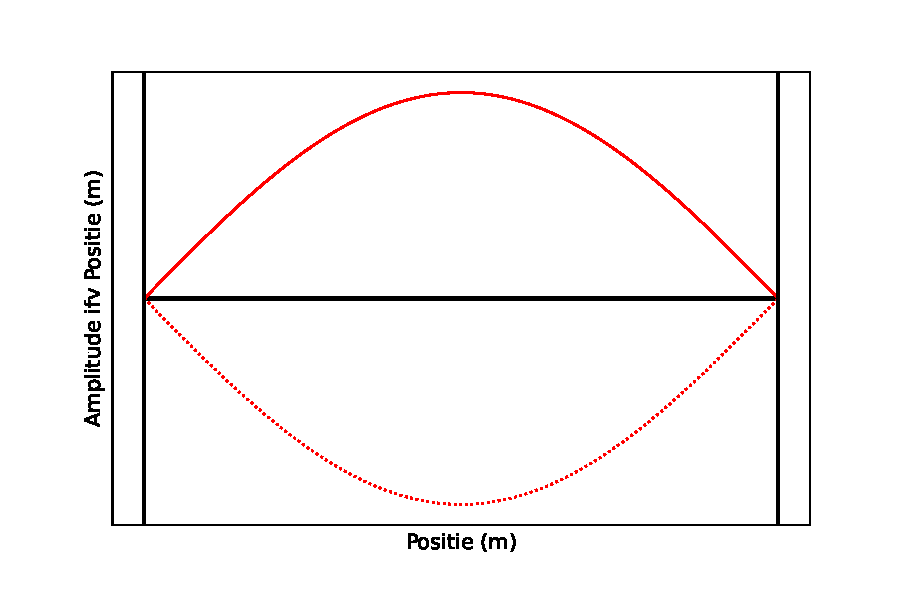
\includegraphics[width=0.7\linewidth]{Eerste_harm}
	\caption[Eerste harmonische]{Eerste harmonische}
	\label{fig:eersteharm}
\end{figure}\\
Hierbij is $m = 1$ dus moet $\lambda = 2L$ en de frequentie is dan $f = \frac{v}{\lambda} = \frac{v}{2L}$.\\
\newpage
\textbf{Tweede harmonische $(m = 2)$}\\
\begin{figure}[h]
	\centering
	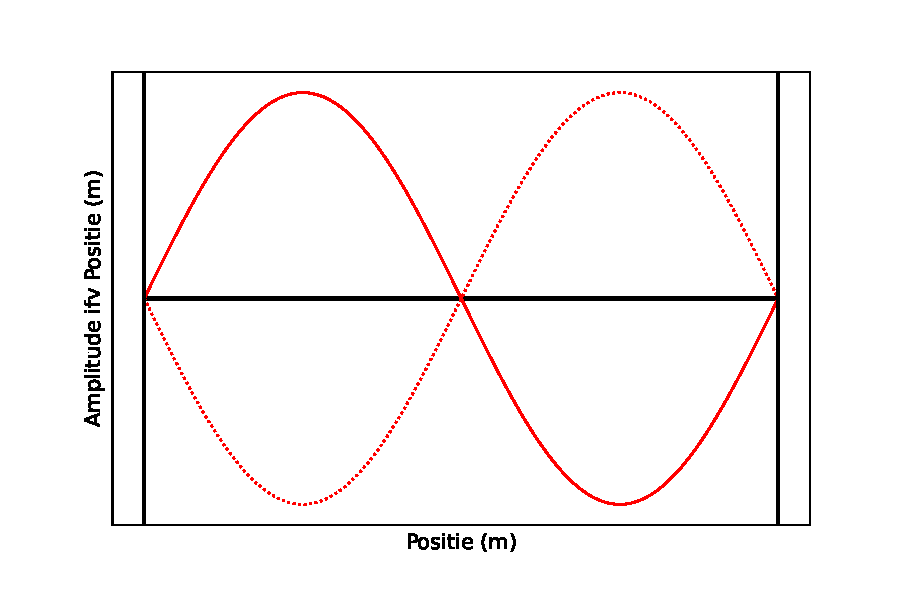
\includegraphics[width=0.7\linewidth]{Tweede_harm}
	\caption[Tweede harmonische]{Tweede harmonische}
	\label{fig:tweedeharm}
\end{figure}\\
Hierbij is $m = 2$ dus moet $\lambda = L$ en de frequentie is dan $f = \frac{v}{\lambda} = \frac{v}{L}$.\\
\textbf{Derde harmonische $(m = 3)$}\\
\begin{figure}[h]
	\centering
	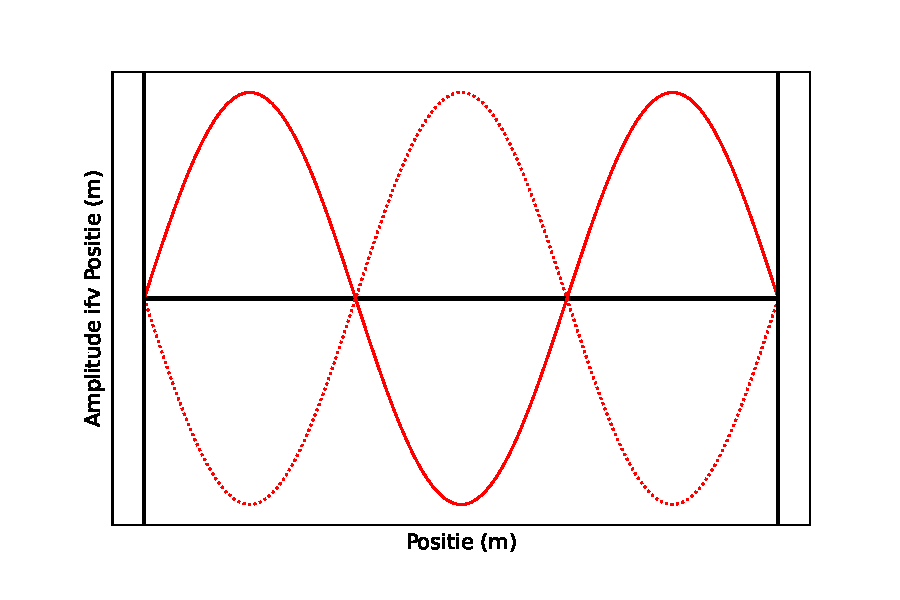
\includegraphics[width=0.7\linewidth]{Derde_harm}
	\caption[Derde harmonische]{Derde harmonische}
	\label{fig:Derdeharm}
\end{figure}\\
Hierbij is $m = 3$ dus moet $\lambda = \frac{2}{3}L$ en de frequentie is dan $f = \frac{v}{\lambda} = \frac{3v}{2L}$.\\
\newpage
\section{Afleiding 12}
\textbf{Energie transport in een golf}\\
\begin{figure}[h]
	\centering
	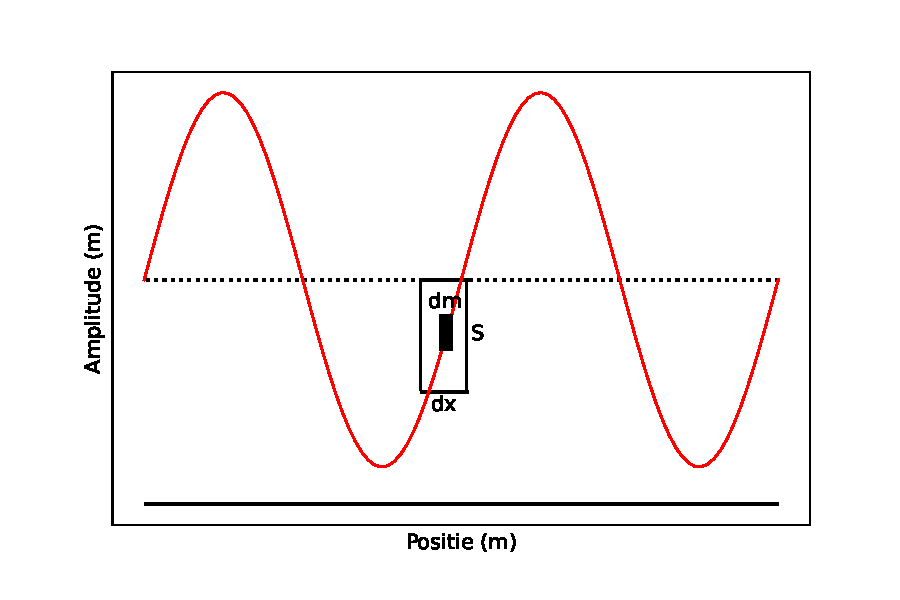
\includegraphics[width=0.7\linewidth]{EnergieGolf}
	\caption[Energie transport]{Energie transport}
	\label{fig:energietransport}
\end{figure}\\
De energie in een massa-veer-systeem is:
\begin{equation*}
	E = \frac{1}{2}kA^2 = dE = \frac{1}{2}\omega^2dmA^2
\end{equation*}
We gebruiken nu het feit dat $\omega = \sqrt{\frac{k}{m}} $ en $\omega = \pi f$:
\begin{equation*}
	dE = 2\pi^2f^2dmA^2
\end{equation*}
We kunnen $dm$ herschrijven als $dm = \rho sdx = \rho sdtv$:
\begin{align*}
	dE &= 2\pi^2f^2A^2\rho Svdt\\
	\frac{dE}{dt} &= 2\pi^2f^2A^2\rho Sv = P
\end{align*}
We bekomen het vermogen van de golf. We kunnen hieruit vervolgens de intensiteit $I$ halen:
\begin{equation*}
	I = \frac{P}{S} = 2\pi^2f^2A^2\rho v
\end{equation*}
\newpage
\section{Afleiding 13}
\textbf{Eigenschappen geluid}\\
\begin{figure}[h]
	\centering
	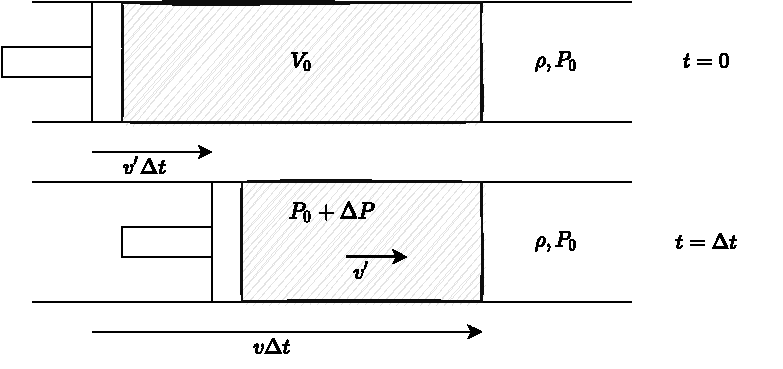
\includegraphics[width=0.7\linewidth]{EigenschappenGeluid}
	\caption[Zuiger]{Drukgolf in een zuiger}
	\label{fig:drukgolfzuiger}
\end{figure}\\
Met $v'$ de snelheid van de zuiger en $v$ de geluidsnelheid kunnen we stellen dat:
\begin{align*}
	V_0 &=Sv\Delta t\\
	\Delta V &= -Sv'\Delta t
\end{align*}
De kracht is dan:
\begin{align*}
	F_{\text{net}} &= (P_0+\Delta P)S-P_0S\\
	F_{\text{net}}&= \Delta PS
\end{align*}
Als we rekening houden met het feit dat $dm=\rho V_0$ kunnen we met behulp van impuls berekenen dat:
\begin{align*}
	F_{\text{net}} \Delta t &=dmv'\\
	F_{\text{net}}\Delta t &= \rho v\Delta tSv'\\
	\Delta PS &= \rho vsv'\\
	\Delta P &= \rho vv'
\end{align*}
\newpage
\section{Afleiding 14}
\textbf{Wiskundige beschrijving van geluid}\\
\begin{figure}[h]
	\centering
	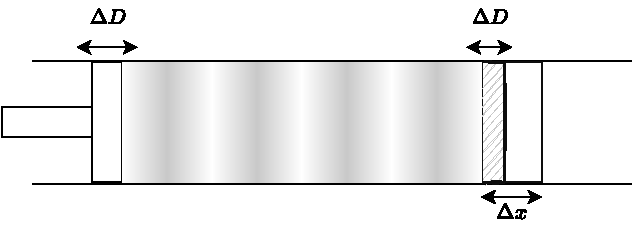
\includegraphics[width=0.7\linewidth]{WiskundigeBeschrijving}
	\caption[Drukgolven]{Drukgolven in een buis}
	\label{fig:drukgolvenbuis}
\end{figure}\\
\begin{figure}[h]
	\centering
	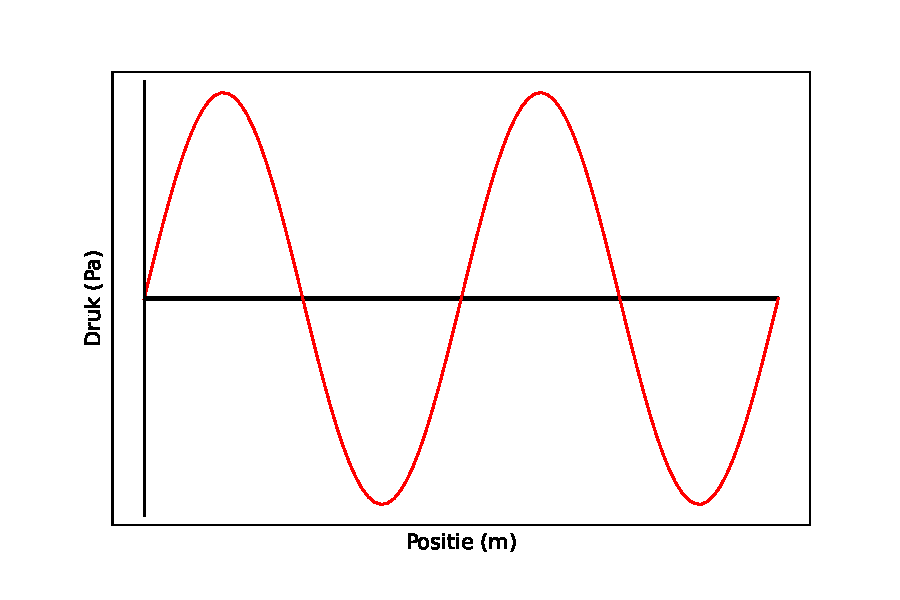
\includegraphics[width=0.5\linewidth]{Drukinbuis}
	\caption[Drukgolven]{Drukgolven in een buis}
	\label{fig:drukgolvenbuisgrafiek}
\end{figure}\\

Met de compressie- of bulk-modulus $B = \frac{\Delta P}{\frac{\Delta V}{V_0}}$ kunnen we zeggen dat:
\begin{align*}
	\Delta P &= -B \frac{\Delta V}{dv}\\
	\Delta P &= -B \frac{\Delta DS}{\Delta xS}\\
	\Delta P &= -B \frac{\partial D}{\partial x}
\end{align*}
We geven een voorstel voor $D$: $D = \Delta sin(kx\pm \omega t)$
\begin{align*}
	\Delta P &= -BAkcos(kx\pm \omega t)\\
	&= -\rho v^2Akcos(kx\pm \omega t)\\
	&= -\rho v\omega Acos(kx\pm \omega t)\\
	&= \underbrace{-2\pi\rho vfA}_{\Delta P_m} cos(kx\pm \omega t)
\end{align*}
\newpage
\section{Afleiding 15}
\textbf{Trillende lucht kolommen}\\
We modelleren de verplaatsing van lucht als:
\begin{equation}
	\label{eq:Verplaatsing}
	D = Asin(kx\pm\omega t)
\end{equation}
De druk kunnen we schrijven als:
\begin{align}
	\Delta P &= -\Delta P_M cos(kx\pm\omega t)\\
	\label{eq:Druk}
	&= -\Delta P_M sin(kx\pm\omega t-\frac{\pi}{2})
\end{align}
Uit vergelijking \ref{eq:Verplaatsing} en \ref{eq:Druk} kunnen we afleiden dat de druk een faseverschil van $\frac{\pi}{2}$ heeft tegenover de verplaatsing zoals te zien is in figuur \ref{fig:faseverschildrukverplaatsing}. 
\begin{figure}[h]
	\centering
	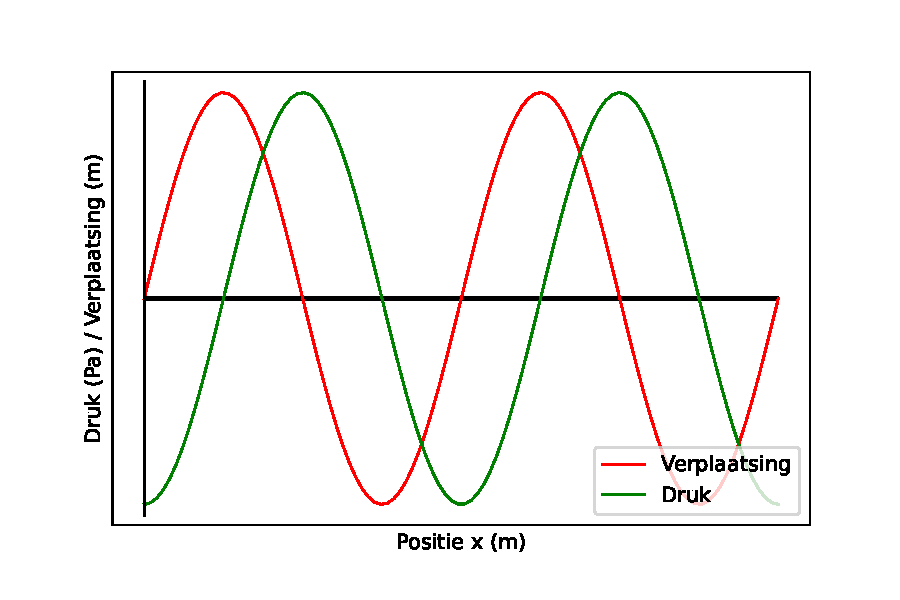
\includegraphics[width=0.7\linewidth]{FaseVerschilDrukVerplaatsing}
	\caption[Fase vershil druk verplaatsing]{Fase verschil tussen druk en verplaatsing}
	\label{fig:faseverschildrukverplaatsing}
\end{figure}
We zien hier duidelijk dat de druk na ijlt op de verplaatsing. 
\newpage
\section{Afleiding 16}
\textbf{Staande golven in een open buis}\\
We veronderstellen een open buis met lengte L. Als nevenvoorwaarde stellen we dat de druk aan de uiterste kanten van de buis gelijk is aan de atmosferische druk $P_{atm}$. We kijken eerst naar de drukverdeling in de buis:
\begin{align*}
	\Delta P_S (x,t) &= \Delta P_m sin(kx+\omega t) + \Delta P_m sin(kx-\omega t)\\
	&= 2\Delta P_m sin(kx)cos(\omega t)
\end{align*}
Hierbij gebruiken we de \href{https://nl.wikipedia.org/wiki/Lijst_van_goniometrische_gelijkheden#Som-naar-product-identiteiten_(regels_van_Simpson)}{regels van Simpson}. Vervolgens kijken we naar de verplaatsing in de buis:
\begin{align*}
	D_S(x,t)&=Asin(kx+\omega t+\frac{\pi}{2})+Asin(kx-\omega t+\frac{\pi}{2})\\
	&= 2Asin(kx+\frac{\pi}{2})cos(\omega t)
\end{align*}
Hierbij gebruiken we nogmaals de \href{https://nl.wikipedia.org/wiki/Lijst_van_goniometrische_gelijkheden#Som-naar-product-identiteiten_(regels_van_Simpson)}{regels van Simpson}.\\
Enkele oplossingen zien er als volgt uit:\\

\textbf{Eerste harmonische}\\
Hierbij is $\lambda = 2L$ en $f=\frac{v}{2L}$.

\begin{figure}[h]
	\centering
	\begin{subfigure}{.5\textwidth}
		\centering
		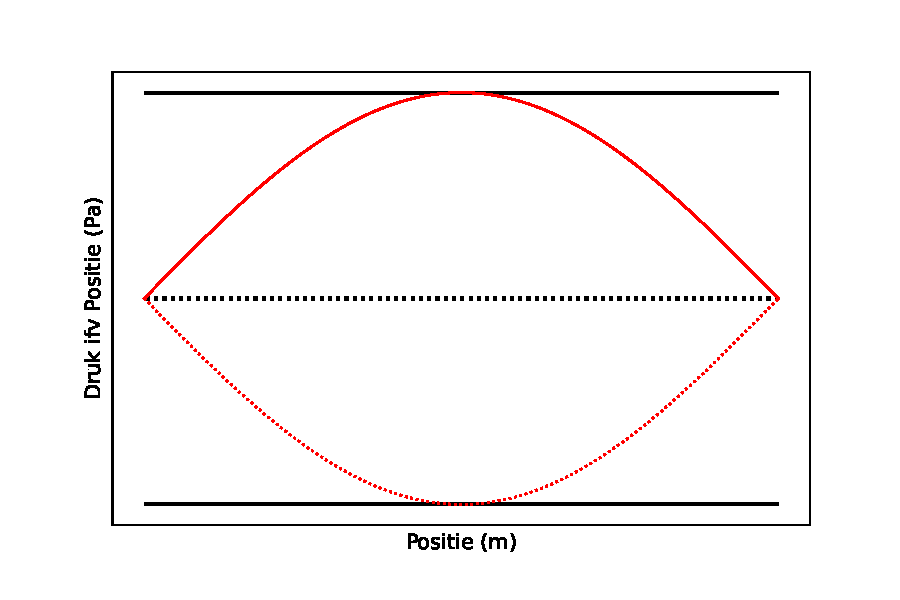
\includegraphics[width=1\linewidth]{OpenBuisEersteDruk}
		\caption{Drukverdeling}
		\label{fig:EersteBuisDruk}
	\end{subfigure}%
	\begin{subfigure}{.5\textwidth}
		\centering
		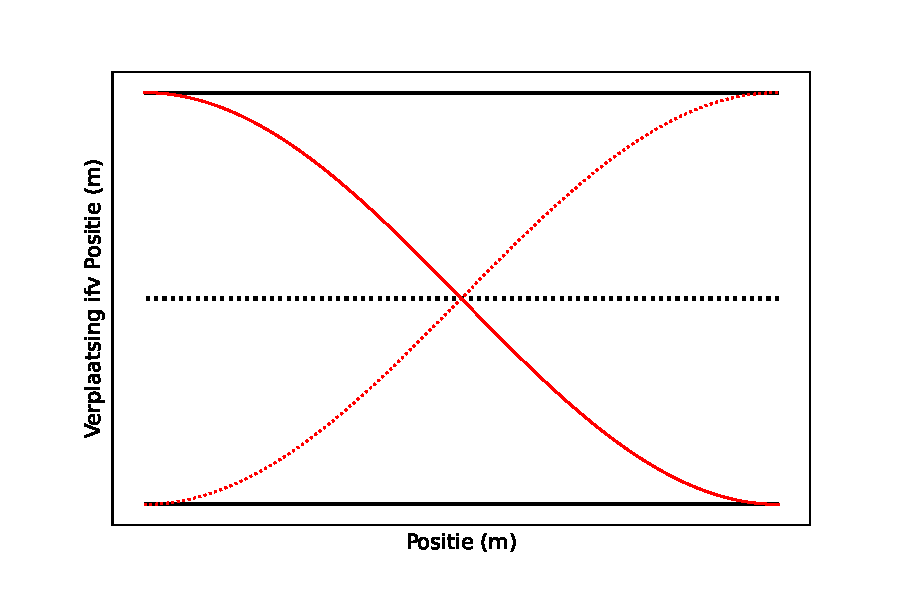
\includegraphics[width=1\linewidth]{OpenBuisEersteVerplaatsing}
		\caption{Verplaatsing}
		\label{fig:EersteBuisVerplaatsing}
	\end{subfigure}
	\caption{Druk en verplaatsing voor de eerste harmonische in een open buis}
	\label{fig:OpenBuisEerste}
\end{figure}
\newpage
\textbf{Tweede harmonische}\\
Hierbij is $\lambda = L$ en $f=\frac{v}{L}$.

\begin{figure}[!h]
	\centering
	\begin{subfigure}{.5\textwidth}
		\centering
		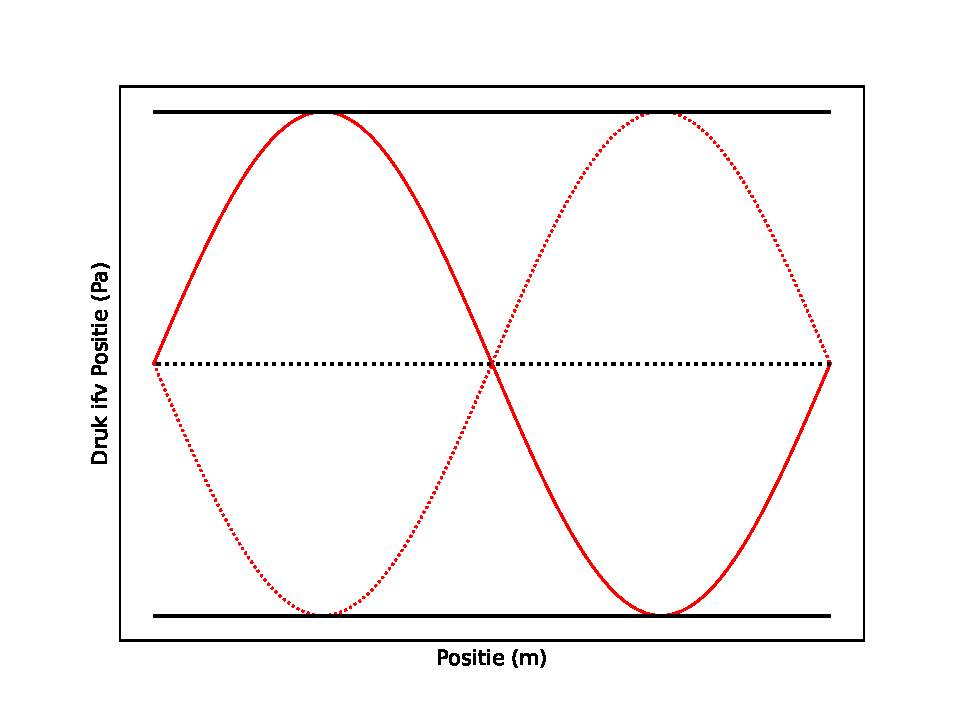
\includegraphics[width=1\linewidth]{OpenBuisTweedeDruk}
		\caption{Drukverdeling}
		\label{fig:TweedeBuisDruk}
	\end{subfigure}%
	\begin{subfigure}{.5\textwidth}
		\centering
		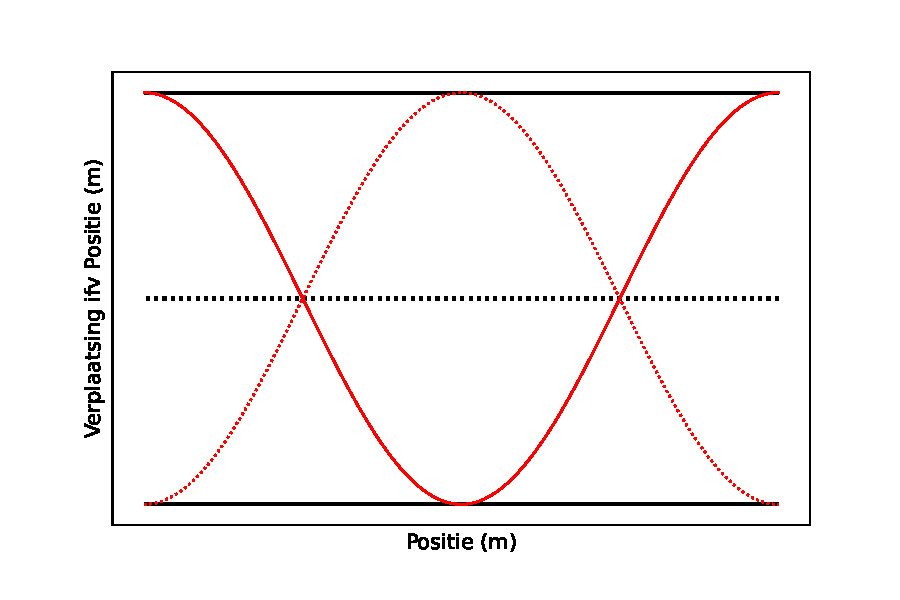
\includegraphics[width=1\linewidth]{OpenBuisTweedeVerplaatsing}
		\caption{Verplaatsing}
		\label{fig:TweedeBuisVerplaatsing}
	\end{subfigure}
	\caption{Druk en verplaatsing voor de tweede harmonische in een open buis}
	\label{fig:OpenBuisTweede}
\end{figure}

\textbf{Derde harmonische}\\
Hierbij is $\lambda = \frac{2L}{3}$ en $f=\frac{3v}{2L}$.

\begin{figure}[!h]
	\centering
	\begin{subfigure}{.5\textwidth}
		\centering
		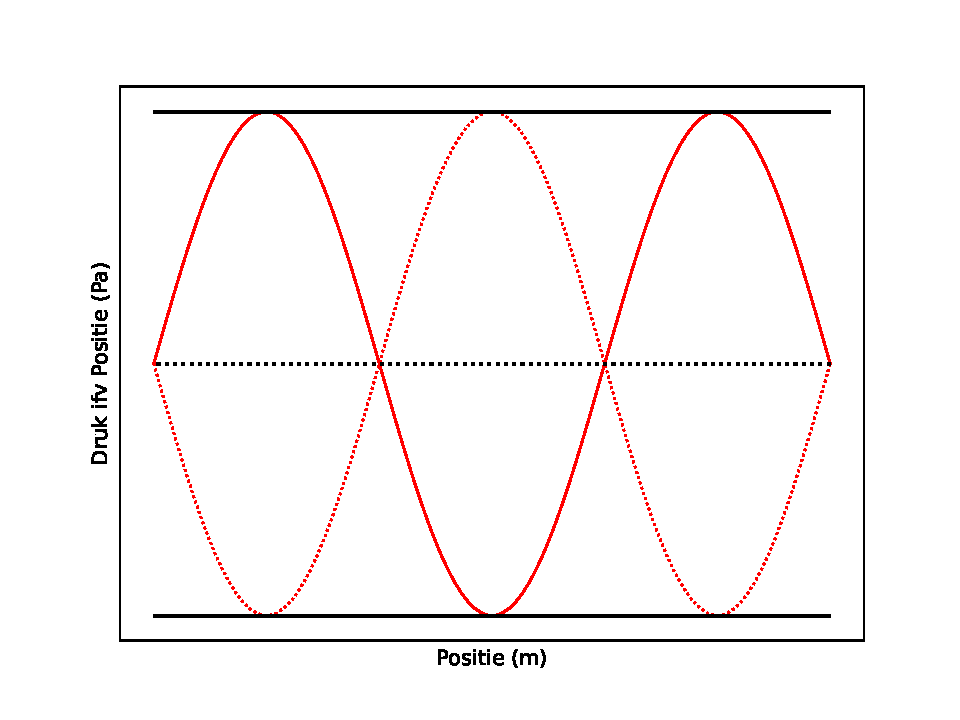
\includegraphics[width=1\linewidth]{OpenBuisDerdeDruk}
		\caption{Drukverdeling}
		\label{fig:DerdeBuisDruk}
	\end{subfigure}%
	\begin{subfigure}{.5\textwidth}
		\centering
		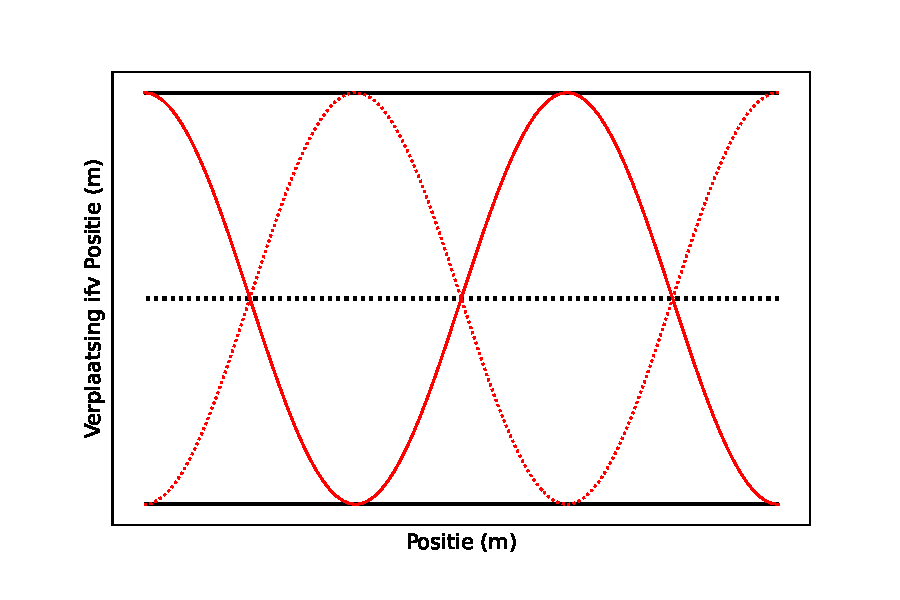
\includegraphics[width=1\linewidth]{OpenBuisDerdeVerplaatsing}
		\caption{Verplaatsing}
		\label{fig:DerdeBuisVerplaatsing}
	\end{subfigure}
	\caption{Druk en verplaatsing voor de derde harmonische in een open buis}
	\label{fig:OpenBuisDerde}
\end{figure}
\newpage
\section{Afleiding 17}
\textbf{Staande golven in een half open buis}\\
\begin{figure}[!h]
	\centering
	\begin{subfigure}{.5\textwidth}
		\centering
		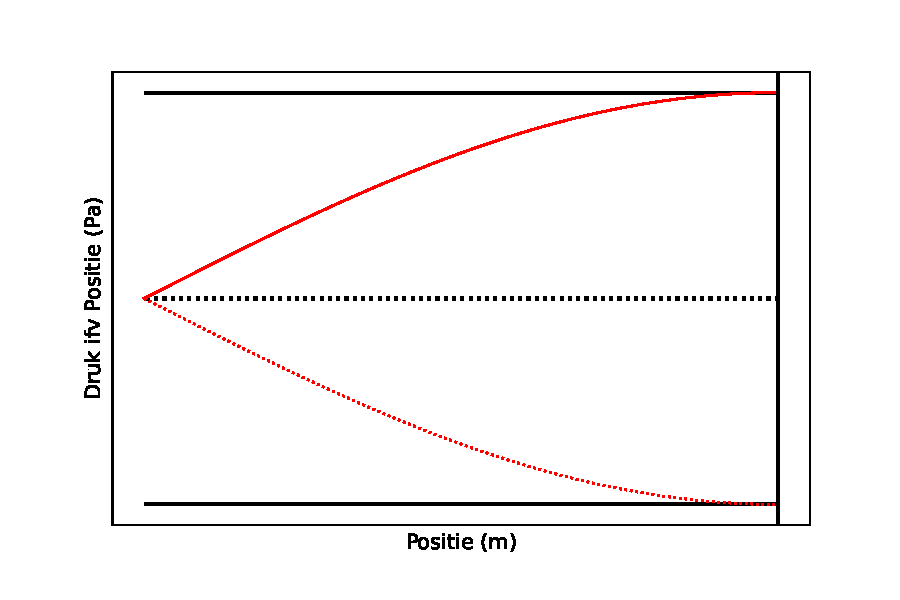
\includegraphics[width=1\linewidth]{HalfOpenBuisEersteDruk}
		\caption{Drukverdeling}
		\label{fig:EersteHalfBuisDruk}
	\end{subfigure}%
	\begin{subfigure}{.5\textwidth}
		\centering
		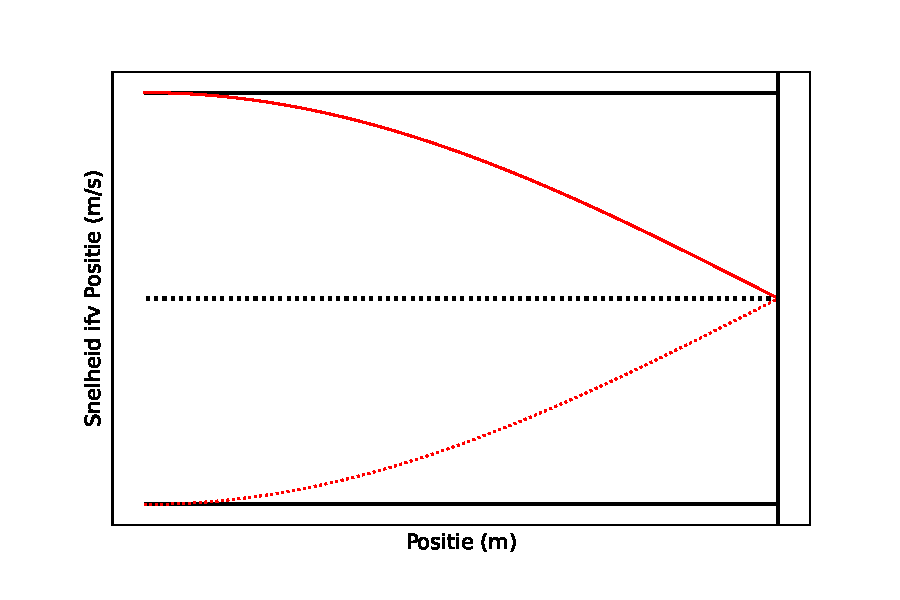
\includegraphics[width=1\linewidth]{HalfOpenBuisEersteSnelheid}
		\caption{Snelheid}
		\label{fig:EersteHalfBuisSnelheid}
	\end{subfigure}
	\caption{Druk en snelheid voor de eerste harmonische in een half open buis}
	\label{fig:HalfOpenBuisEerste}
\end{figure}\\
We kunnen opnieuw enkele randvoorwaarden stellen:
\begin{equation*}
	D_s(L,t)=0\Rightarrow kl+\frac{\pi}{2} = \pi
\end{equation*}
Dit wil zeggen dat:
\begin{equation*}
	k=\frac{\pi}{2L}=\frac{2\pi}{\lambda}\Rightarrow \lambda=4L \wedge f=\frac{v}{4L}
\end{equation*}
We kunnen ook een tweede nevenvoorwaarde opstellen:
\begin{equation*}
	kL+\frac{\pi}{2}=2\pi
\end{equation*}
Dit wil zeggen dat:
\begin{equation*}
	k=\frac{3\pi}{2L}=\frac{2\pi}{\lambda}\Rightarrow \lambda=\frac{4L}{3} \wedge f=\frac{3v}{4L}
\end{equation*}
\newpage
\section{Afleiding 18}
\textbf{Interferentie van geluidsgolven}\\
\begin{figure}[h]
	\centering
	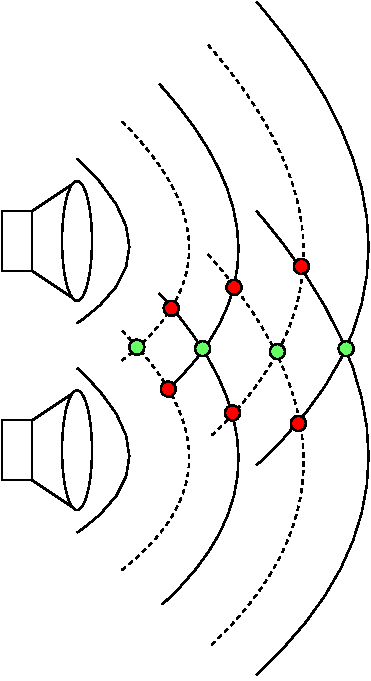
\includegraphics[width=0.3\linewidth,angle=90]{InterferentieSpeakers}
	\caption[Interferentie]{Interferentie bij speakers}
	\label{fig:interferentiespeakers}
\end{figure}
\begin{figure}[h]
	\centering
	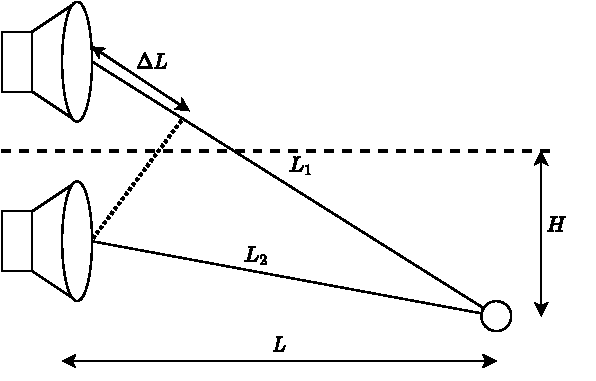
\includegraphics[width=0.5\linewidth]{SpeakersWiskundig}
	\caption[Interferentie wiskundig]{Interferentie wiskundig}
	\label{fig:speakerswiskundig}
\end{figure}\\
We kunnen de druk beschrijven als:
\begin{align*}
	\Delta P_1 &= \Delta P_msin(kL_1\pm\omega t)\\
	\Delta P_2 &= \Delta P_msin(kL_2\pm\omega t)
\end{align*}
Door beide op te tellen en de regels van Simpson toe te passen krijgen we:
\begin{equation*}
	\Delta P = 2\Delta P_msin(k\frac{L_1+L_2}{2}\pm\omega t)cos(k\frac{L_1-L_2}{2})
\end{equation*}
We onderscheiden 2 soorten interferentie zoals te zien in figuur \ref{fig:interferentiespeakers}. Constructieve interferentie (groen) en destructieve interferentie (rood).

Bij constructieve interferentie is $\frac{k\Delta L}{2}=0,\pi,2\pi,\ldots$ Dit wil zeggen dat $\Delta L$ moet voldoen aan $\Delta L = 0,\lambda,2\lambda,\ldots$. Destructieve interferentie doet zich voor als $\frac{k\Delta L}{2}=\frac{\pi}{2},\frac{3\pi}{2},\ldots$. $\Delta L$ moet hier dus voldoen aan $\Delta L = \frac{\lambda}{2},\frac{3\lambda}{2},\ldots$.

\newpage
\section{Afleiding 19}
\textbf{Kloppen van een golf}\\
Als 2 golven frequenties hebben die zeer dicht bij elkaar liggen, krijgen we kloppingen. We kunnen de druk van beide golven voorstellen als:
\begin{align*}
	D_1&=Asin(2\pi f_1t)\\
	D-2&=Asin(2\pi f_2t)
\end{align*}
Door beide op te tellen en de regels van Simpson toe te passen krijgen we:
\begin{equation*}
	D=2Acos(2\pi\frac{f_1-f_2}{2}t)sin(2\pi\frac{f_1+f_2}{2}t)
\end{equation*}
Hierbij vermelden we ook nog dat als $f_1\approx f_2\Rightarrow\Delta\omega=\frac{f_1-f_2}{2}<<1$.


\newpage
\section{Afleiding 20}
\textbf{Doppler effect}\\
Het doppler effect doet zich voor als de bron en waarnemer van een geluid in beweging zijn tegenover elkaar. We analyseren nu het geval waarin de bron beweegt: als de bron naar rechts beweegt,  zal een waarnemer die zich links bevindt een lagere frequentie waarnemen. Een waarnemer die rechts staat, zal daarentegen een hogere frequentie waarnemen. De nieuwe frequentie heet $\lambda'$. Wiskundig kunnen we $\lambda'$ bepalen met volgende redenering:
\begin{equation*}
	\lambda'=\lambda\pm v_{bron}T=\lambda\pm v_{bron}\frac{\lambda}{v_s}=\lambda(1\pm\frac{v_{bron}}{v_s})
\end{equation*}
De nieuwe frequentie is dan $f'=\frac{f}{1\pm\frac{v_{bron}}{v_s}}$.
\begin{center}
	\begin{tabular}{|c|c|}
		\hline
		Bron naar je toe  & f$\nearrow$ \\
		\hline
		Bron van je weg & f $\searrow$\\
		\hline
	\end{tabular}
	
\end{center}
\newpage
\section{Afleiding 21}
\textbf{Basiswetten voor elektromagnetische golven}\\
\paragraph{Wet van Ampère}
\begin{equation*}
	\oint\vec{B}\vec{dl}=\mu I_{\text{lus}}+\mu_0\epsilon_0\frac{d\Phi_E}{dt}
\end{equation*}
waarbij $\Phi_E$ de elektrische flux is:
\begin{figure}[h]
	\centering
	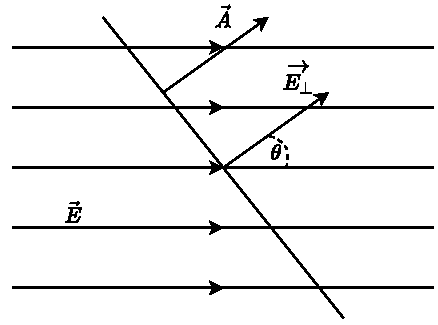
\includegraphics[width=0.5\linewidth]{ElektrischVeld}
	\caption[Elektrisch veld]{Elektrisch veld}
	\label{fig:elektrischveld}
\end{figure}
\begin{align*}
	\Phi_E &= E_{\perp}A\\
	&= Ecos(\theta)A\\
	&= \vec{E}\cdot\vec{A}\quad\text{(Scalair product)}
\end{align*}
\paragraph{Wetten van maxwell}
\begin{align}
	\oint\vec{E}\vec{dA}&=\frac{Q}{\epsilon_0}\\
	\oint\vec{B}\vec{dA}&=0\\
	\label{eq:faraday}
	\oint\vec{E}\vec{dl}&=-\frac{\partial\Phi_B}{\partial t}\\
	\label{eq:maxwell}
	\oint\vec{B}\vec{dl}&=\mu\epsilon_0\frac{\partial\Phi_E}{\partial t}
\end{align}
waarbij vergelijking \ref{eq:faraday} en \ref{eq:maxwell} invloed hebben op elektromagnetische golven.
\newpage
\section{Afleiding 22}
\textbf{Generatie EM golven}\\
Men kan elektromagnetische golven genereren door twee platen naast elkaar te zetten met een wisselspanningsbron zoals in figuur \ref{fig:emgolf1}:
\begin{figure}[h]
	\centering
	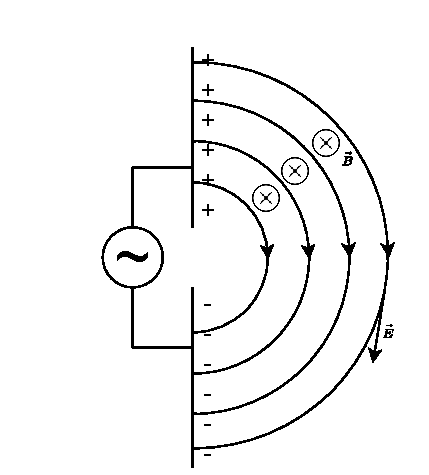
\includegraphics[width=0.3\linewidth]{EMGolf1}
	\caption[Generatie]{Generatie EM golf}
	\label{fig:emgolf1}
\end{figure}\\
Als de spanningsbron van polariteit veranderd, veranderen ook de velden van richting zoals in figuur \ref{fig:emgolf2}. Hier kunnen we tevens ook zien hoe de golf zich voortplant in de ruimte: na verloop van tijd zullen de golven een lineair karakter krijgen. 
\begin{figure}[h]
	\centering
	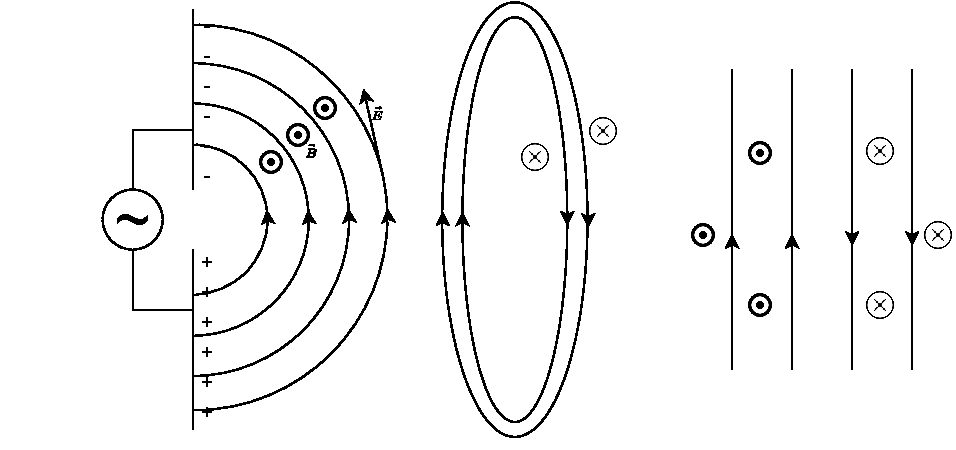
\includegraphics[width=0.7\linewidth]{EMGolf2}
	\caption[Generatie en voortplanting]{Generatie en voortplanting EM golf}
	\label{fig:emgolf2}
\end{figure}
\newpage
\section{Afleiding 23}
\textbf{Elektromagnetische velden}\\
Eerst enkele eigenschappen van elektromagnetische golven
\begin{enumerate}
	\item $\vec{B}$ en $\vec{E}$ staan loodrecht op de voortplantingsrichting (transversale golven)
	\item $\vec{B}$ staat loodrecht op $\vec{E}$
	\item $\vec{B} \times\vec{E}$ geeft de voortplantingsrichting van de golf
	\item $\vec{B}$ en $\vec{E}$ zijn harmonische golven met $\Delta\Phi = 0$
\end{enumerate}
\begin{figure}[h]
	\centering
	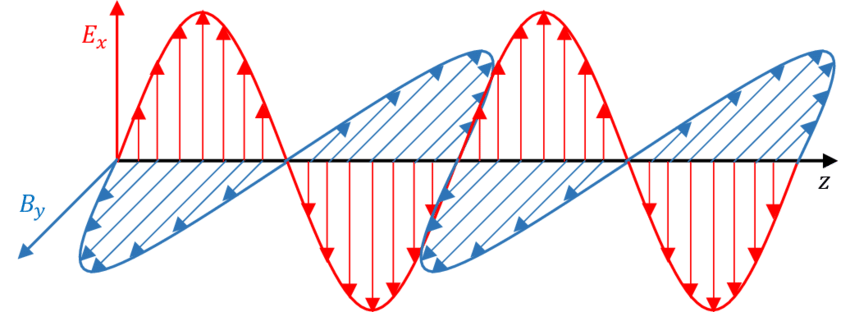
\includegraphics[width=0.7\linewidth]{An-electromagnetic-wave}
	\caption[Elektromagnetische golf]{Elektromagnetische golf}
	\label{fig:an-electromagnetic-wave}
\end{figure}
In figuur \ref{fig:an-electromagnetic-wave} kunnen we stellen dat:
\begin{align*}
	\vec{E} &= E_msin(kx-\omega t)\vec{j}\\
	\vec{B} &= B_msin(kx-\omega t)\vec{k}
\end{align*}
\end{document}
